%\documentclass{beamer}
\documentclass[handout]{beamer}
\usetheme{boxes} 
%\usetheme{default}

%math fonts
%\renewcommand\mathfamilydefault{\rmdefault}

%page numbers
\setbeamertemplate{footline}[page number]
\setbeamertemplate{section in head/foot}{\hfill\insertsectionheadnumber.~\insertsectionhead}
\setbeamertemplate{section in head/foot shaded}{\color{structure!50}\hfill\insertsectionheadnumber.~\insertsectionhead}
\setbeamertemplate{section in toc}{\inserttocsectionnumber.~\inserttocsection}

\setbeamercovered{invisible}
\setbeamertemplate{navigation symbols}{} 
\usepackage{mathtools}
\usepackage{graphicx}
\usepackage{amsmath}
\usepackage{epstopdf}
\usepackage{color}
\usepackage{hyperref}

\title{Total Least Squares and applications in Table Tennis}
\author{Okan Ko\c{c}}
\institute[IAS]
{
MPI for Intelligent Systems, T\"ubingen \\
Robot Learning Lab \\
\medskip
{\emph{okan.koc@tuebingen.mpg.de}}
}
\date{\today}

% Set the paths where all figures are taken from:
\graphicspath{{Pictures/}}
\mathtoolsset{showonlyrefs} 
\newcommand{\includesvg}[1]{%
% \executeiffilenewer{#1.svg}{#1.pdf}%
% {inkscape -z -D --file=#1.svg %
% --export-pdf=#1.pdf --export-latex}%
 \input{#1.pdf_tex}%
}
\AtBeginSection{\frame{\sectionpage}}

\begin{document}
%
\begin{frame}
\titlepage
\end{frame}
%
\begin{frame}
\frametitle{Table of Contents}
\tableofcontents
\end{frame}
%
\section{Least Squares}
%
\begin{frame}{Least Squares}
\begin{itemize}
\item $X \in \mathbb{R}^{m \times n}$ is the design matrix
\item $y \in \mathbb{R}^{m}$ is the observations vector
\item $\beta \in \mathbb{R}^{n}$ is the parameter vector to be estimated
\item $X\beta \approx y$
\item $r = y - X\beta$ are the residuals 
\item Recast Least Squares as 
%
\begin{equation}
\begin{aligned}
\text{minimize} &\ r^{\mathrm{T}}Wr \\
\text{subject to} &\ y + r \in \text{Range}(X)
\end{aligned}
\end{equation}
%
\end{itemize}
\end{frame}
%
\begin{frame}{General Linear Model}
\begin{itemize}
\item Recast as $XB \approx Y$, $Y \in \mathbb{R}_{m \times k}$
\item $R = Y - XB$ is the residuals matrix
\item Same normal equations with Frobenius norm:
\begin{equation}
\begin{aligned}
\text{minimize} &\ \|W^{1/2}R\|_{F} \\
\text{subject to} &\ Y + R \in \text{Range}(X)
\end{aligned}
\end{equation}
\item $\hat{B} = (X^{\mathrm{T}}WX)^{-1}X^{\mathrm{T}}WY$
\end{itemize}
\end{frame}
%
\section{Total Least Squares (TLS)}
%
\begin{frame}{An errors-in-variables model}
\begin{itemize}
\item What happens when the design matrix is also not precise?
\item $(X + E)B = Y + R$
\item Optimization with this model (no weighting)
\begin{equation}
\begin{aligned}
\text{minimize} &\ \|\begin{bmatrix} E & R\end{bmatrix}\|_{F} \\
\text{subject to} &\ Y + R \in \text{Range}(X + E)
\end{aligned}
\end{equation}
\item Is there a (closed form) solution?
\end{itemize}
\end{frame}
%
\begin{frame}{Solution to TLS}
\begin{itemize}
\item Is there a (closed form) solution?
\item No! In general it fails to have a solution.
\item Example:
\begin{equation}
\begin{aligned}
X = \begin{bmatrix}
   1 & 0 \\ 0 & 0
 \end{bmatrix}, \ Y = \begin{bmatrix}
 1 \\ 1
 \end{bmatrix} 
\end{aligned}
\end{equation}
\item For every $\epsilon > 0$, $Y \in \text{Range}(X + E_{\epsilon}), \ E_{\epsilon} = \begin{bmatrix} 0 & 0 \\ 0 & \epsilon \end{bmatrix}$
\end{itemize}
\end{frame}
%
\begin{frame}{SVD Solution to TLS}
\begin{itemize}
\item Rewrite $(X + E)B = Y + R$ as  
\begin{equation}
\begin{aligned}
\begin{bmatrix} X+E & Y+R \end{bmatrix} \begin{bmatrix} B \\ -I_k \end{bmatrix} = 0 \\
\end{aligned}
\end{equation}
\item Using Eckart-Young theorem
\begin{equation}
\begin{aligned}
\begin{bmatrix} X & Y \end{bmatrix} = \begin{bmatrix} U_X & U_Y \end{bmatrix} \begin{bmatrix} \Sigma_X & 0 \\ 0 & \Sigma_Y \end{bmatrix} \begin{bmatrix} V_{XX} & V_{XY} \\ V_{YX} & V_{YY} \end{bmatrix}^{\mathrm{T}} \\
\begin{bmatrix} X+E & Y+R \end{bmatrix} = \begin{bmatrix} U_X & U_Y \end{bmatrix} \begin{bmatrix} \Sigma_X & 0 \\ 0 & 0_k \end{bmatrix} \begin{bmatrix} V_{XX} & V_{XY} \\ V_{YX} & V_{YY} \end{bmatrix}^{\mathrm{T}}
\end{aligned}
\end{equation}
 
\end{itemize}
\end{frame}
%
\begin{frame}{SVD Solution to TLS}
\begin{itemize}
\item After subtracting and manipulating (or simply believing me)
\begin{equation}
\begin{aligned}
\hat{B}_{tls} &= -V_{XY}V_{YY}^{-1} \\
\hat{E} &= U_X \Sigma_X V_{XX}^{\mathrm{T}} - X
\end{aligned}
\end{equation}
\item Many extensions: global, structured, truncated $\ldots$
\begin{equation}
\begin{aligned}
\hat{B}_{ttls} = -V_{XY}V_{YY}^{\dagger}
\end{aligned}
\end{equation}
\begin{figure}
\centering
\includegraphics[width=0.4\textwidth]{LSvsTLS.jpg}%
\caption{Total Least Squares minimizes in 1D the sum of the squared perpendicular distances.}
\end{figure}
\end{itemize}
\end{frame}
%
\begin{frame}{Truncated TLS in MATLAB}
\begin{figure}
\centering
\includegraphics[scale=0.2, angle= 0]{ttls.jpg}			
\caption{Truncated TLS in MATLAB}
\end{figure}
\end{frame}
%
\section{Applications in Robotic Table Tennis}
%
\begin{frame}{Application 1: Iterative Learning Control}
\begin{itemize}
\item Linearize nominal robot dynamics $\dot{x} = f(x,u)$ around a trajectory $s$ to predict errors $e = x - s$
\begin{equation}
\begin{aligned}
e \approx Fu + d
\end{aligned}
\end{equation}
\item Compute every iteration the feedforward compensation signal $u$ to drive error $e$ to $0$
\begin{equation}
\begin{aligned}
u = -F^{\dagger}d
\end{aligned}
\end{equation}
\item However robot dynamics may not be known well! Try to take this into account with TLS!
\begin{equation}
\begin{aligned}
u_{TLS}, \ \delta F &= \arg\min_{u,\delta F} \|\begin{bmatrix}E & r \end{bmatrix} \|_{F} \\
E &= \delta F \\
r &= -d - (F + \delta F)u
\end{aligned}
\end{equation}
\end{itemize}
\end{frame}
%
\begin{frame}{Simulation results}
\begin{itemize}
\item ILC with pseudoinverse: ILC cannot approach trajectory very well, and after 8 iterations starts to diverge.
\end{itemize}
\begin{figure}
\centering
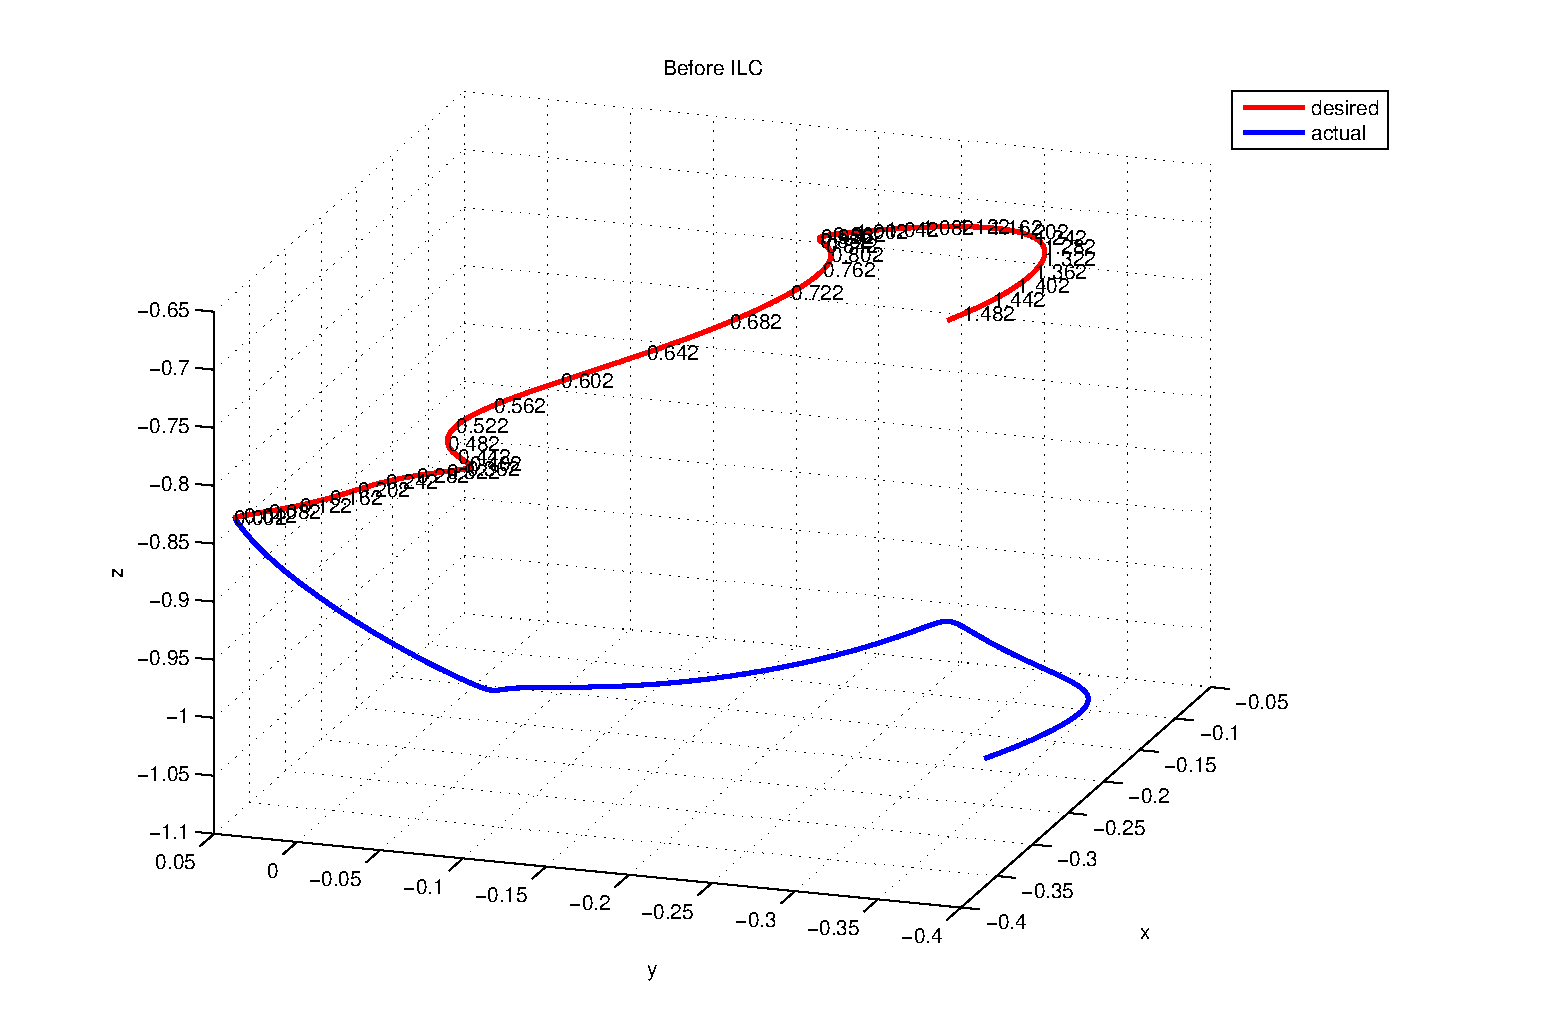
\includegraphics[width=0.5\textwidth]{beforeILC.eps}%
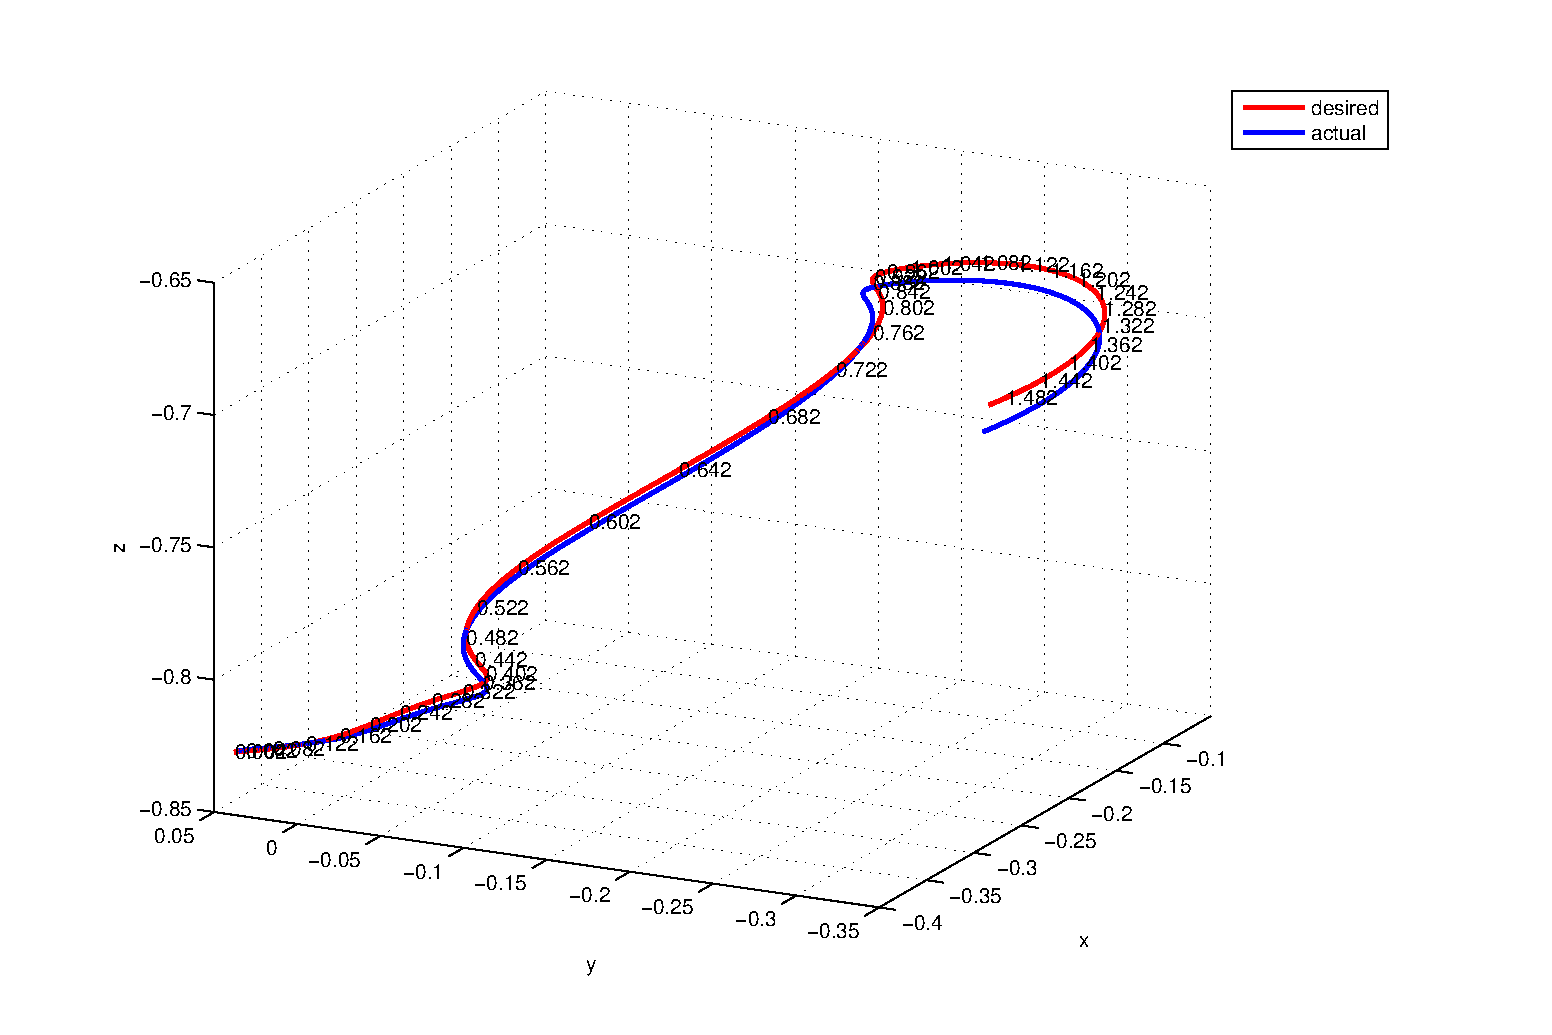
\includegraphics[width=0.5\textwidth]{afterILCPseudoInv.eps}		
\caption{Before and after applying ILC (10 iterations)}
\end{figure}
\end{frame}
%
\begin{frame}{Simulation results}
\begin{itemize}
\item ILC with total least squares: ILC approaches the trajectory very well, and shows excellent tracking performance.
\end{itemize}
\begin{figure}
\centering
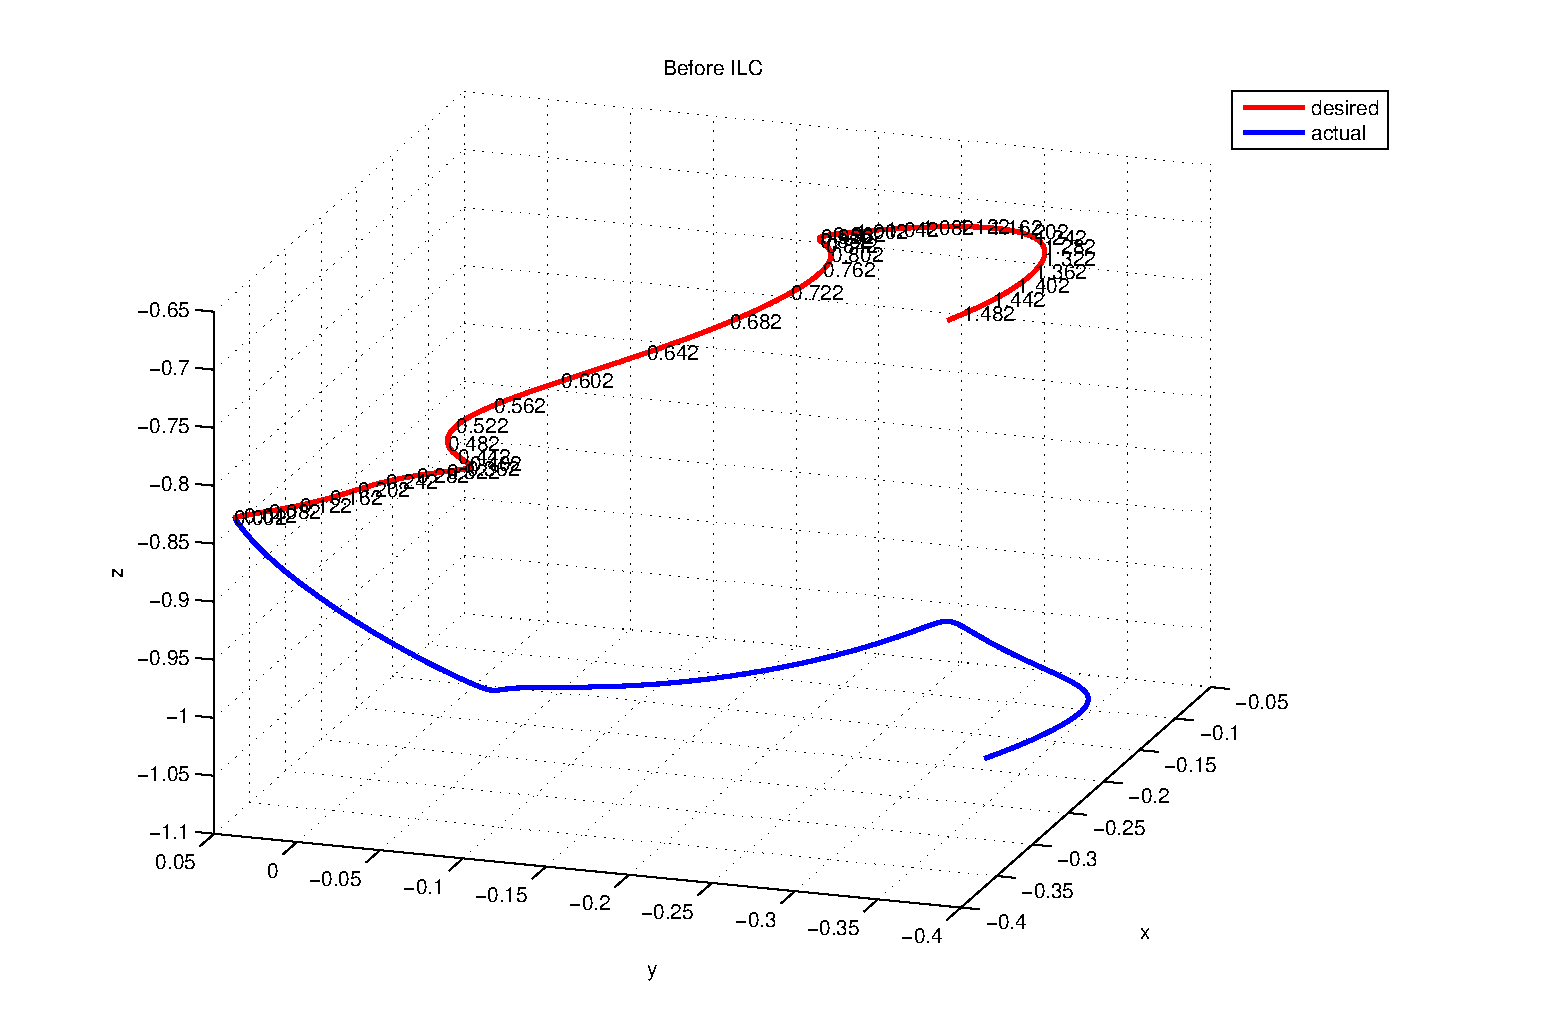
\includegraphics[width=0.5\textwidth]{beforeILC.eps}%
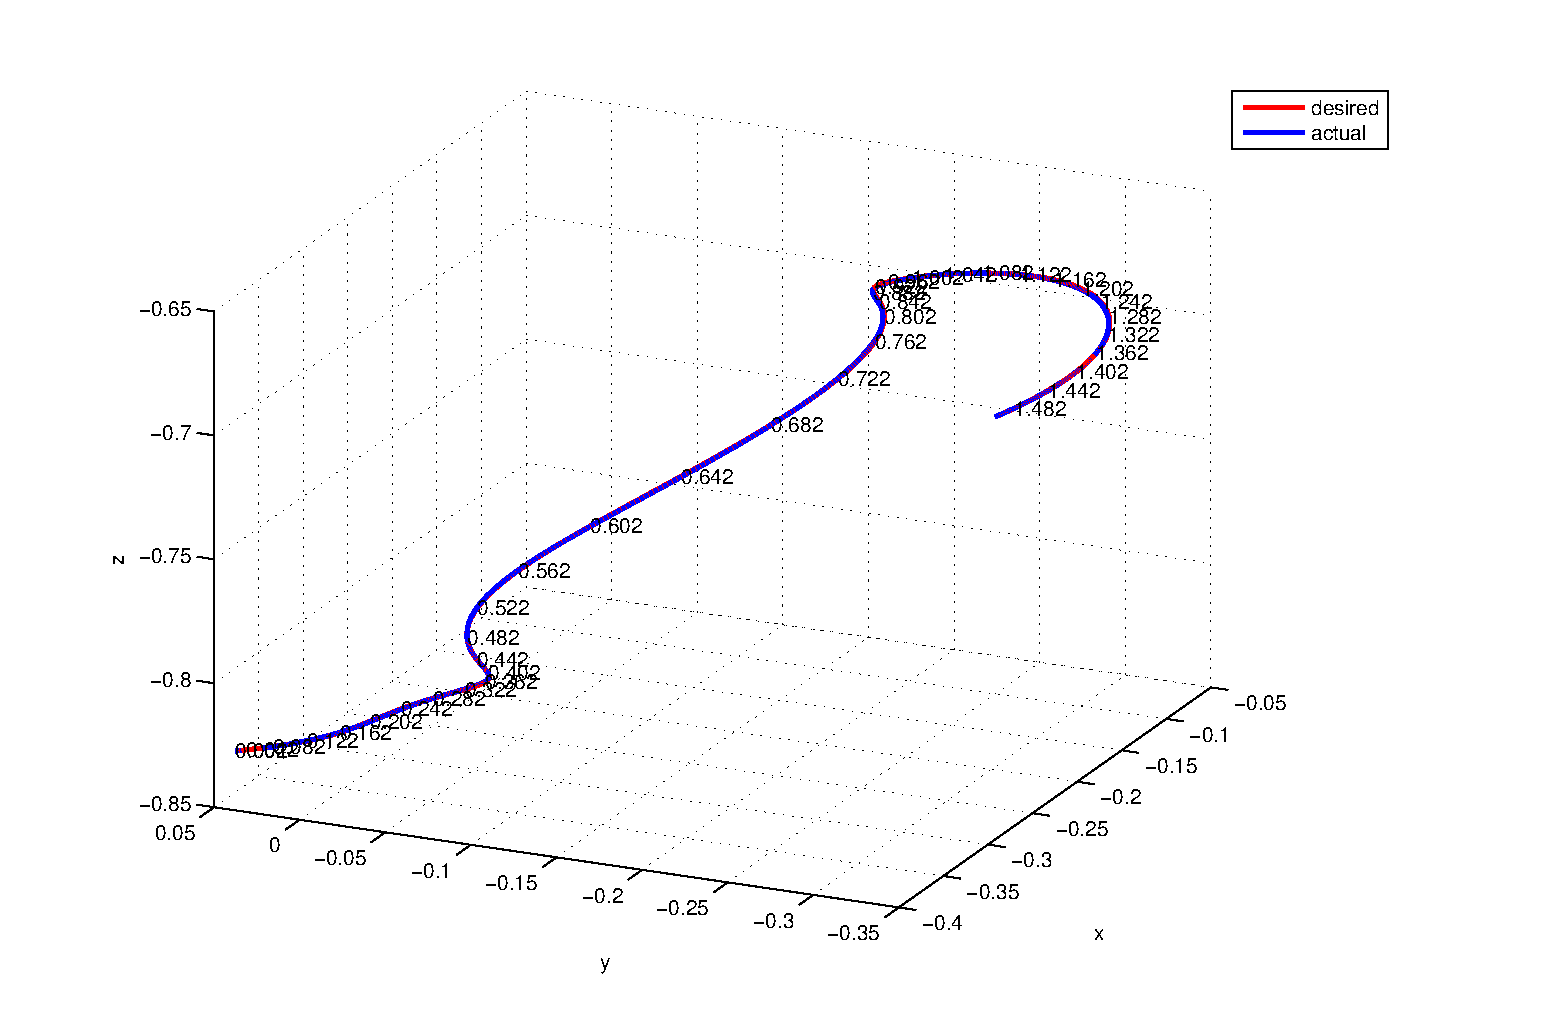
\includegraphics[width=0.5\textwidth]{afterILCTLS.eps}		
\caption{Before and after applying ILC (10 iterations)}
\end{figure}
\end{frame}
%
\begin{frame}{Application 2: Ball Prediction}
\begin{itemize}
\item Take into account the fact that the time information as well as the triangulation provided by the cameras are not exact!
\item How to apply it precisely? Does it fit into the framework of robust Kalman filters?
\end{itemize}
\begin{figure}
\centering
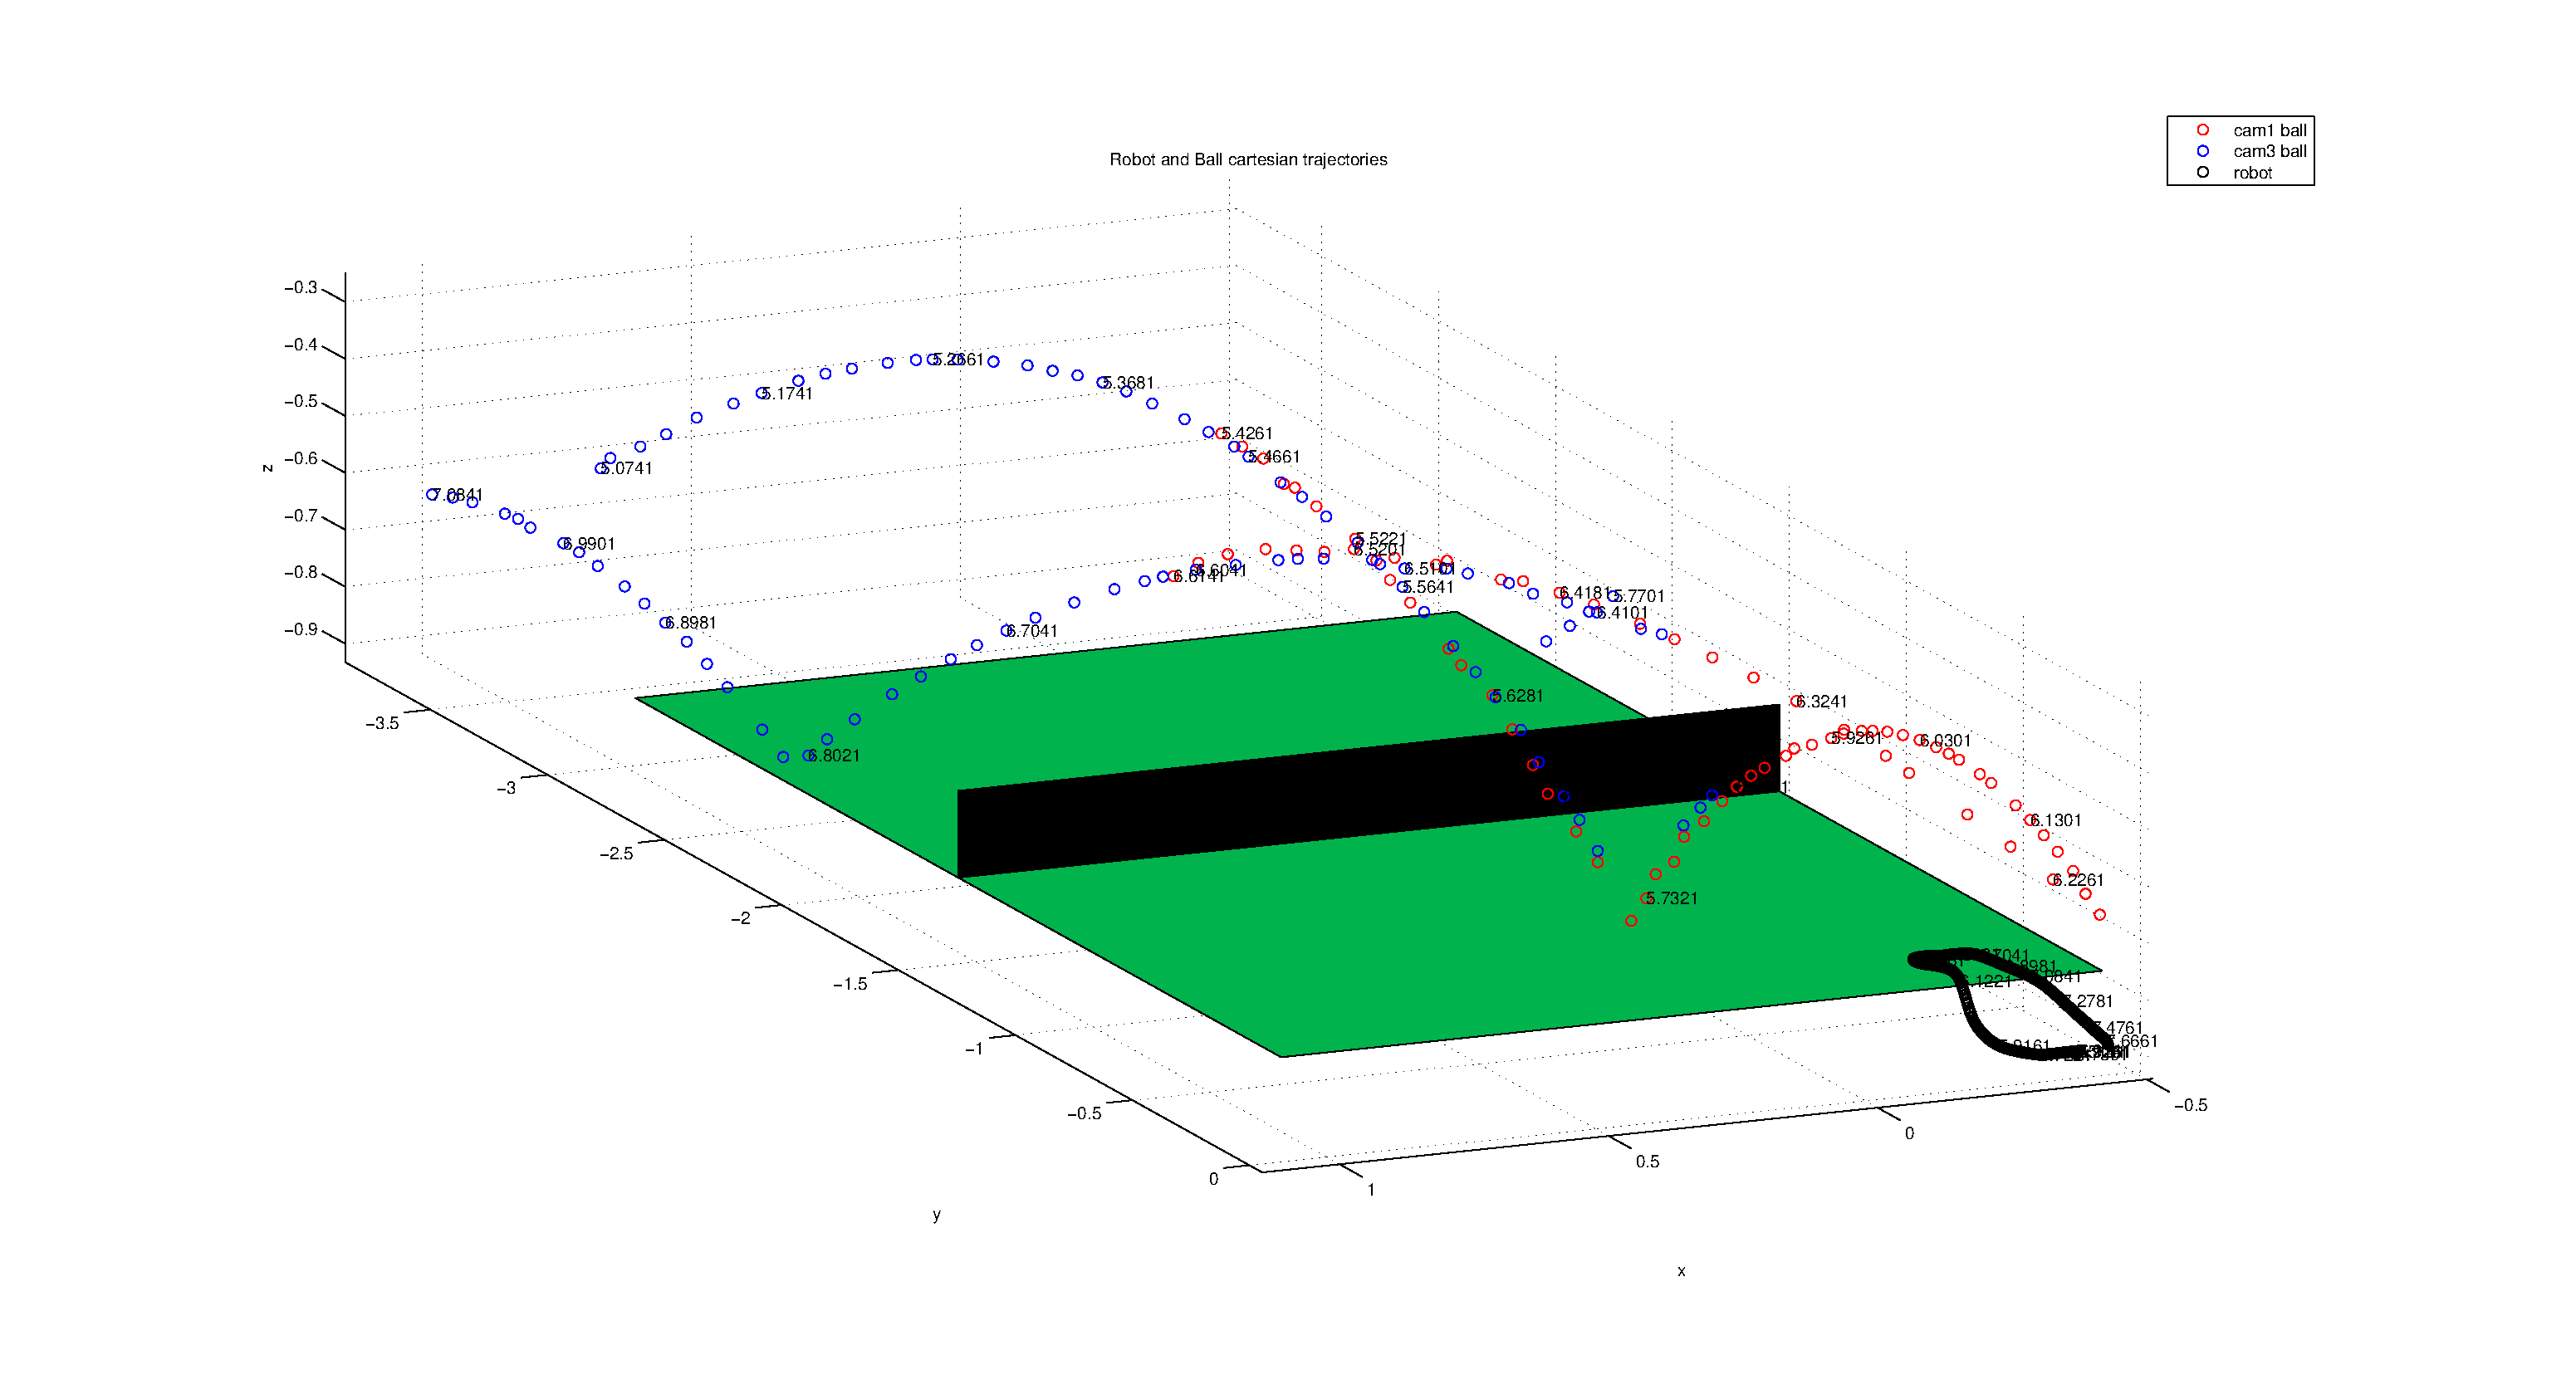
\includegraphics[width=0.9\textwidth]{ballPrediction.eps}%	
\caption{Ball rebound trajectory should be estimated robustly so that the robot can intercept the ball and return it at least to the opponent's court.}
\end{figure}
\end{frame}
%
\begin{frame}{Extensions}
\begin{itemize}
\item We can use \emph{nonlinear truncated total} least squares for ILC if we linearize the robot dynamics in every iteration.
\item We know that the structure of the model errors $\delta F$ is block lower diagonal. Can we incorporate it in the weighting? 
\item \emph{Kernelize all things}: structured nonlinear truncated kernel total least squares!
\end{itemize}
\end{frame}

\section{References}
\begin{frame}[allowframebreaks]{References}
\nocite{*}
\def\newblock{\hskip .11em plus .33em minus .07em}
\bibliographystyle{alpha}
\bibliography{myReferences} % file name of the bibtex
\end{frame}
%

\end{document} 